\section{تئوری موسیقی}

تئوری موسیقی، زبان توصیف قطعات موسیقی‌ست و همانند زبان طبیعی، قواعد و قوانین خاصی دارد.

\subsection{نت}

\begin{figure}
	\centering
	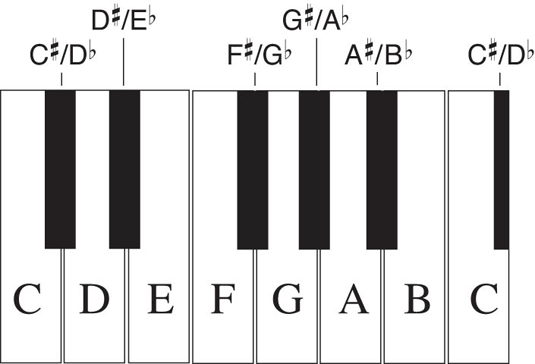
\includegraphics[scale=0.4]{figures/pianokeys.jpg}
	% To make sure citation doesn't appear in list of figures
	\caption {
	نت‌های روی کلیدهای یک پیانو
	}
	\label{fig:pianokeys}
\end{figure}


پایه‌ای‌ترین جز یک قطعه موسیقی، نت
\fnote{Note}
نام دارد. 

اصوات، موج‌های مکانیکی‌ای هستند که از ارتعاش ذرات هوا تشکیل شده‌اند. هرگاه این ارتعاش فرکانس بالاتری داشته باشد، مغز انسان صدا را به عنوان صدایی زیر تر، و هروقت ارتعاش فرکانس کندتری باشد، صدا را به عنوان صدایی بم‌تر تشخیص می‌دهد.
نت‌ها، ارتعاشاتی با فرکانس‌های معین هستند. اکثریت قریب به اتفاقات موسیقی‌های تولید شده تا به امروز، از تنها ۱۲ نت تشکیل شده‌اند، چرا که طبق تجربه، سیستم شنوایی انسان این ۱۲ نت را آهنگین‌تر و منظم‌تر می‌داند.
به طور خلاصه‌تر،  هرگاه که نسبت فرکانس نت‌هایی که  کنار هم پخش می‌شوند، به کسرهای ساده نزدیک‌تر باشند، نت‌های متفاوت در کنار هم آهنگین‌تر به نظر می‌رسند، منظور از کسرهای ساده، کسرهایی‌ست که در هنگام نوشته‌شدن به صورت اعشاری، اعشار کم‌تری داشته‌باشند.

در یک پیانو، نت‌ها بر روی کلیدهای آن قرار گرفته‌اند و در شکل
\ref{fig:pianokeys}
قابل مشاهده هستند.
نت کلیدهای سفید پیانو از حرف 
$A$
تا
$G$
نام‌گذاری شده‌اند. 
نت کلیدهای سیاه، با توجه به نت کلیدهای سفید نام‌گذاری شده‌اند و نام‌های آن‌ها شامل علائم
$\sharp$
و
$\flat$
هستند. 
به این معنا که از چپ به راست، نت کلید سیاهی که بعد از یک کلید سفید آمده، اسم نت آن کلید سفید به علاوه‌ی یک
$\sharp$
را می‌گیرد؛ و در عین حال، نام کلید سفید قبلی‌اش به علاوه‌ی یک
$\flat$
را نیز می‌گیرد. پس به عنوان مثال، نت کلید سیاهی که بین کلیدهای سفید 
$F$
و 
$G$
قرار گرفته، 
$F\sharp$
یا
$G\flat$
نام دارد.

\subsection{پرده و نیم‌پرده}
جابه‌جایی از هر نت به نت بعدی آن، یک نیم‌پرده
\fnote{Half-step}
نام دارد. در اکثر جابه‌جایی‌ها، این نیم‌پرده به معنای رفتن از هر نت
$X$
به نت
$X\sharp$
است؛ اما بین جفت نت‌های
$B, C$
و
$E, F$
نت میانی‌ای وجود ندارد، پس یک نیم‌پرده در این جفت نت‌ها، به معنای رفتن به نت بعدی است.
با همین منطق، جابه‌جایی از یک نت به دومین نت بعد از آن، یک پرده
\fnote{Whole step}
نام دارد.

\subsection{اکتاو}
همان‌طور که گفته شد، در موسیقی ۱۲ نت وجود دارد؛ اما تقریبا همه‌ی آلات موسیقی بیش‌تر از ۱۲ حالت برای نواختن نت‌ها دارند. به عنوان مثال در پیانو، این امر این‌گونه ممکن می‌شود که اگر فرکانس یک نت را دو برابر کنیم، به نتی می‌رسیم که نام همان نت را دارد، اما یک اکتاو
\fnote{Octave}
بالاتر است.

طبق قضیه‌ی ریشه‌ی گویا
\fnote{Rational root theorem}
در ریاضیات، به ازای هر دو عدد طبیعی 
$a, b$
و عدد طبیعی
$n$
که بزرگ‌تر از ۱ است، رابطه‌ی زیر هیچ‌گاه برقرار نیست:
\begin{equation}
    (\frac{a}{b})^n \neq 2
\end{equation}
\myequations{قضیه‌ی ریشه‌ی گویا}
به همین علت، در پیانو نسبت فرکانس بین هر دو نت مجاور، 
$2^{\frac{1}{12}}$
است.
برای دیدن چرایی این مساله، نسبت برخی از فرکانس‌های نت‌های مجاور در یک اکتاو و فواصل آن‌ها با کسرهای ساده را بررسی می‌کنیم:

\begin{equation}
\begin{gathered}
    2^{\frac{1}{12}} \approx 1.05946309 \simeq \frac{16}{15} \hst ; \hso error = \hso 0.67\% \\[3pt]
    2^{\frac{2}{12}} \approx 1.12246205 \simeq \frac{9}{8} \hst ; \hso error = \hso 0.67\% \\[3pt]
    2^{\frac{3}{12}} \approx 1.18920712 \simeq \frac{6}{5} \hst ; \hso error = \hso 0.22\% \\[3pt]
    2^{\frac{4}{12}} \approx 1.25992105 \simeq \frac{5}{4} \hst ; \hso error = \hso 0.89\% \\[3pt]
    2^{\frac{5}{12}} \approx 1.33483985 \simeq \frac{4}{3} \hst ; \hso error = \hso 0.79\% \\[3pt]
    2^{\frac{7}{12}} \approx 1.49830708 \simeq \frac{3}{2} \hst ; \hso error = \hso 0.11\% \\[3pt]
    2^{\frac{8}{12}} \approx 1.58740105 \simeq \frac{8}{5} \hst ; \hso error = \hso 0.78\% \\[3pt]
    2^{\frac{9}{12}} \approx 1.68179283 \simeq \frac{5}{3} \hst ; \hso error = \hso 0.90\% \\[3pt]
    2^{\frac{10}{12}} \approx 1.78179744 \simeq \frac{16}{9} \hst ; \hso error = \hso 0.22\% \\[3pt]
\end{gathered}    
\end{equation}
\myequations{نسبت فرکانس‌های یک اکتاو پیانو}

\subsection{
آکورد
}

یک آکورد
\fnote{Chord}
، مجموعه‌ای از نت‌هاست که به صورت تقریبا هم‌زمان نواخته می‌شوند و در کنار هم، صدایی متفاوت تولید می‌کنند.
معمولا آکوردها متشکل از ۳ نت یا بیش‌تر هستند و با اسم اولین نت موجود در آکورد شناخته می‌شوند که به این نت، نت ریشه
\fnote{Root note}
نیز گفته می‌شود این ۳ نت موجود در یک آکورد، می‌توانند هر ۳ نتی باشند،؛ اما لزوما هر ترکیبی از نتها، صدای أهنگینی تولید نخواهد کرد.
به مجموعه‌ی چند آکورد کنار هم، یک سلسله‌آکورد
\fnote{Chord progression}
گفته می‌شود و برخی سلسله‌آکوردها به کرات در موسیقی‌های مختلف تکرار می‌شوند.
آکوردها عمدتا به دو دسته‌ی ماینور
\fnote{Minor chord}
و ماژور
\fnote{Major chord}
تقسیم می‌شوند.

آکوردهای ماژور متشکل از سه نت هستند، ابتدا نت ریشه، سپس نتی که در سه نیم‌گام جلوتر از آن قرار دارد و در آخر نتی که چهار نیم‌گام جلوتر از نت دوم قرار دارد. آکوردهای ماژور عمدتا اصوات شادابی تولید می‌کنند.

آکوردهای ماینور نیز مشابه آکوردهای ماژور هستند، با این تفاوت که نت دوم آن‌ها، چهار نیم‌پرده با نت اول فاصله دارد و نت سوم، سه نیم‌پرده با نت دوم فاصله دارد.
آکوردهای ماینور عمدتا اصوات غم‌گینی تولید می‌کنند.

\subsection{
گام
}
هر گام
\fnote{Scale}
یک گروه از نت‌هاست که هنگام نواخته‌شدن به ترتیبی خاص، صدایی آهنگین تولید می‌کنند. برخلاف آکوردها، قرار دادن هر گروهی از نت‌ها کنار هم، لزوما تشکیل یک گام نمی‌دهد.
گام‌ها، همانند آکوردها با استفاده از اولین نت نواخته‌شده‌شان شناخته می‌شوند و به دو نوع هستند. یکی
گام‌های کروماتیک
\fnote{Chromatic scale}
که هر گام کروماتیک متشکل از ۱۲ نت در یک گام است؛
و دیگری گام دیاتونیک
\fnote{Diatonic scale}
که هر گام دیاتونیک، متشکل از ۷ نت در یک گام است.
هستند که هر کدام از این انواع، زیرشاخه‌های خود را دارند. به عنوان مثال، گام‌های ماژور
\fnote{Major scale}
و گام‌های مینور
\fnote{Minor scale}
از زیرشاخه‌های گام‌های دیاتونیک هستند که گام‌های ماژور، ترتیبی همانند
[پرده-پرده-نیم‌پرده-پرده-پرده-پرده-نیم‌پرده]
و گام‌های ماینور ترتیبی همانند
[پرده-نیم‌پرده-پرده-پرده-نیم‌پرده-پرده-پرده] دارند.
به طور ساده، به گامی که قطعه‌ای را آغاز کند و در قطعه حضور پررنگی داشته‌باشد، کلید
\fnote{Key}
آن قطعه گفته می‌شود و شکل کلی قطعه را تعیین می‌کند.
پس به عنوان مثال، اگر آهنگی در
$A$
ماینور باشد، به این معناست که با نت‌های زیر آغاز شده و این نت‌ها حضور فعالی در طول قطعه دارند:
\begin{equation}
    A, B, C, D, E, F, G, A
\end{equation}
\myequations{گام $A$ ماینور}